\chapter{Estrutura}

\section{Solução}

\subsection{Desenho Industrial}

Utilizou-se o software CATIA V5 para a criação do CAD (\textit{computer aided design}) da estrutura. A estrutura completa e seus módulos separados foram construídos com base nas medidas das caixas comerciais e hastes selecionadas. Além disso, as medidas também foram baseadas para seguir uma proporção com os painéis solares. 

Temos o suporte principal para acoplar dos demais módulos da estrutura que foi chamada de hastes. Elas consistem em dois tubos de aço carbono afastados entre si a uma distancia de 450 mm. Seu desenvolvimento foi pensado de forma a garantir a estabilidade da estrutura, por isso é possível ver a utilização de barras chatas de aço soldadas nas hastes para que a rigidez do sistema aumente.

A caixa superior será o local onde os componentes eletrônicos ficaram. Toda a transferência de dados acontecerá a partir dela. Os componentes vão possuir um espaço de 450x450mm em uma placa de montagem para seus devidos acoplamentos. Um \textit{cooler} será instalado na lateral interna da caixa superior para ajudar na dissipação do calor. Em sua porta será fixado um holofote que servirá de sinal luminoso para o motorista. Ambas as caixas possuem trancas para evitar a abertura de forma a expor os componentes a possíveis danos. 

A caixa inferior será apoiada no chão pois a mesma carregará as baterias que alimentarão energeticamente o sistema. Por questões técnicas, se as baterias ficassem na caixa superior com os componentes eletrônicos, elas poderiam gerar o aquecimento dos mesmos, o que poderia causar o mal funcionamento do sistema por completo, além de gerar um momento maior na base da estrutura devido ao braço de alavanca entre a caixa superior e o chão. A caixa inferior estará ligada através de 4 abraçadeiras do tipo copo às hastes de suporte principal.

O suporte para o acoplamento dos painéis solares se encontra atrás da caixa superior. Este suporte será soldado nas hastes em 4 pontos com uma angulação de 15 graus como solicitado pelo subsistema de energia para melhor captação de luz solar. 

No ponto mais alto da estrutura, a 3 metros do chão, teremos duas componentes de suma importância para o funcionamento do RaDop. As antenas do radar Doppler e a câmera. A câmera possui apenas um grau de liberdade, sendo assim, é necessário que o seu posicionamento na estrutura seja feita de forma correta para garantir a angulação necessária para capturar com eficiência as imagens dos carros. Oposta à câmera e acima da caixa superior teremos duas antenas do radar Doppler. Elas possuirão um suporte que permitirá à elas dois graus de liberdade, visando melhorar o posicionamento das antenas para que a emissão e recepção do sinal sejam feitas da melhor maneira possível.

As plantas geradas a partir do \textit{software} CATIA V5 com detalhes em padrão internacional que foram utilizadas para a construção de todas as peças da parte estrutural se encontram no Apêndice \ref{plantas_construcao} desse relatório, assim como as demais peças que não são do subsistema estrutural mas foram necessárias para dimensionar os módulos estruturais.

\section{Construção do Protótipo}

O projeto será construído através dos recursos disponibilizados pela Universidade de Brasília como o galpão, seu maquinário e os técnicos disponíveis. O aval para a construção de uma fundação de concreto para o radar foi adquirida para melhor funcionamento estrutural do mesmo. As escolhas dos materiais e processos de fabricação foram feitas através do conhecimento prévio adquirido por simulações computacionais. 

\subsection{Projeto dos Componentes Estruturais}

Foram utilizadas no projeto duas caixas de painel de controle (quadro de comando) pois essas possuíam todas as necessidades do projeto, como mostra a Figura \ref{caixa}. As caixas são de aço e possuem 1mm de espessura com dimensões de 500x500x250mm. São rígidas e resistentes a corrosão com tratamento de fosfato de zinco e pintura a pó. Ambas possuem borrachas de vedação hermética e possuem grau de proteção IP54 conforme a ABNT NBR IEC 60529 \cite{involucro}. Cada caixa pesa 10 quilos. A placa de montagem da cor laranja para por os componentes eletrônicos necessários para o funcionamento do RaDop.

\begin{figure}[H]
	\centering
    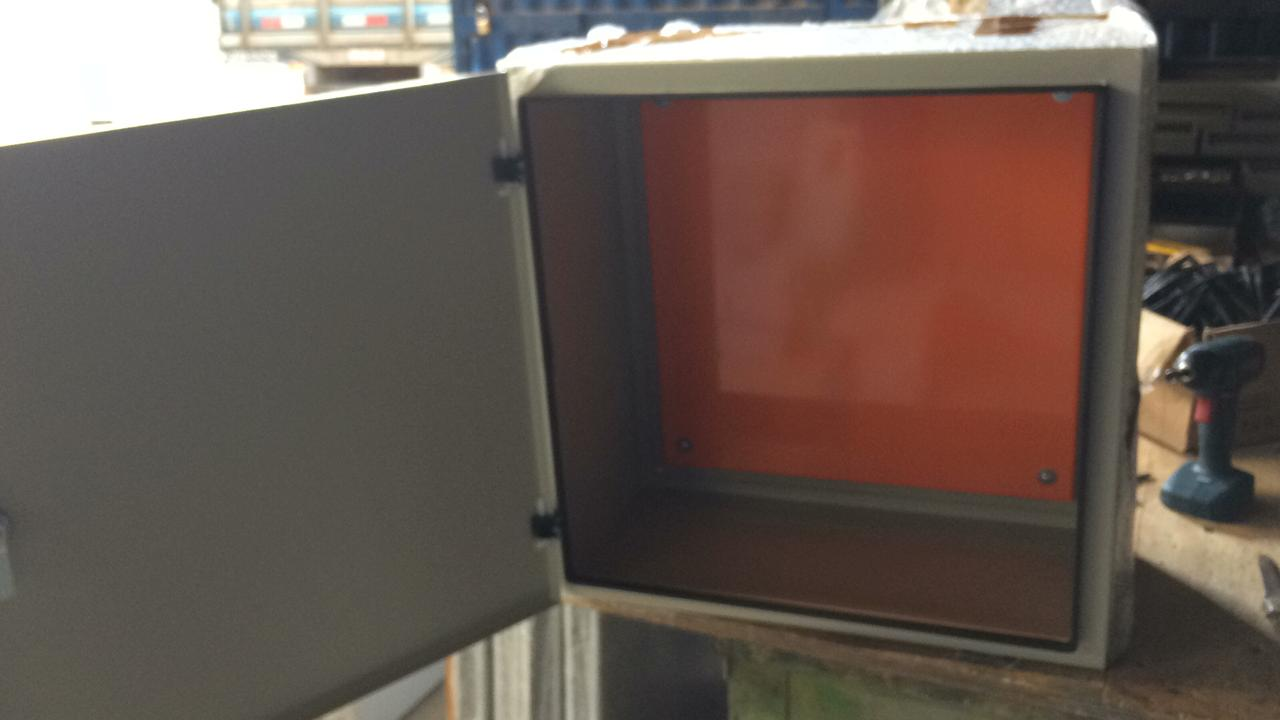
\includegraphics[keepaspectratio=true,scale=0.315]{figuras/caixa.jpg}
    \caption{Caixa de aço utilizada para o projeto.}
    \label{caixa}
\end{figure}

Dois tubos de aço carbono chapa 13 com 2 polegadas de diâmetro (50,80 mm) foram utilizadas para suportar todos os módulos necessários da estrutura, suas dimensões foram selecionadas com base nos cálculos numéricos feitos para medir os esforços e tensões que elas serão submetidas, como mostra a Figura \ref{tubos}. Os tubos também foram selecionadas como base nas suas propriedades de rigidez e o fator comercial também foi algo decisivo na escolha do material. Cada tubo terá 4 metros sendo que 1 metro será utilizado para que a estrutura tenha sua fundação no concreto.

\begin{figure}[H]
	\centering
    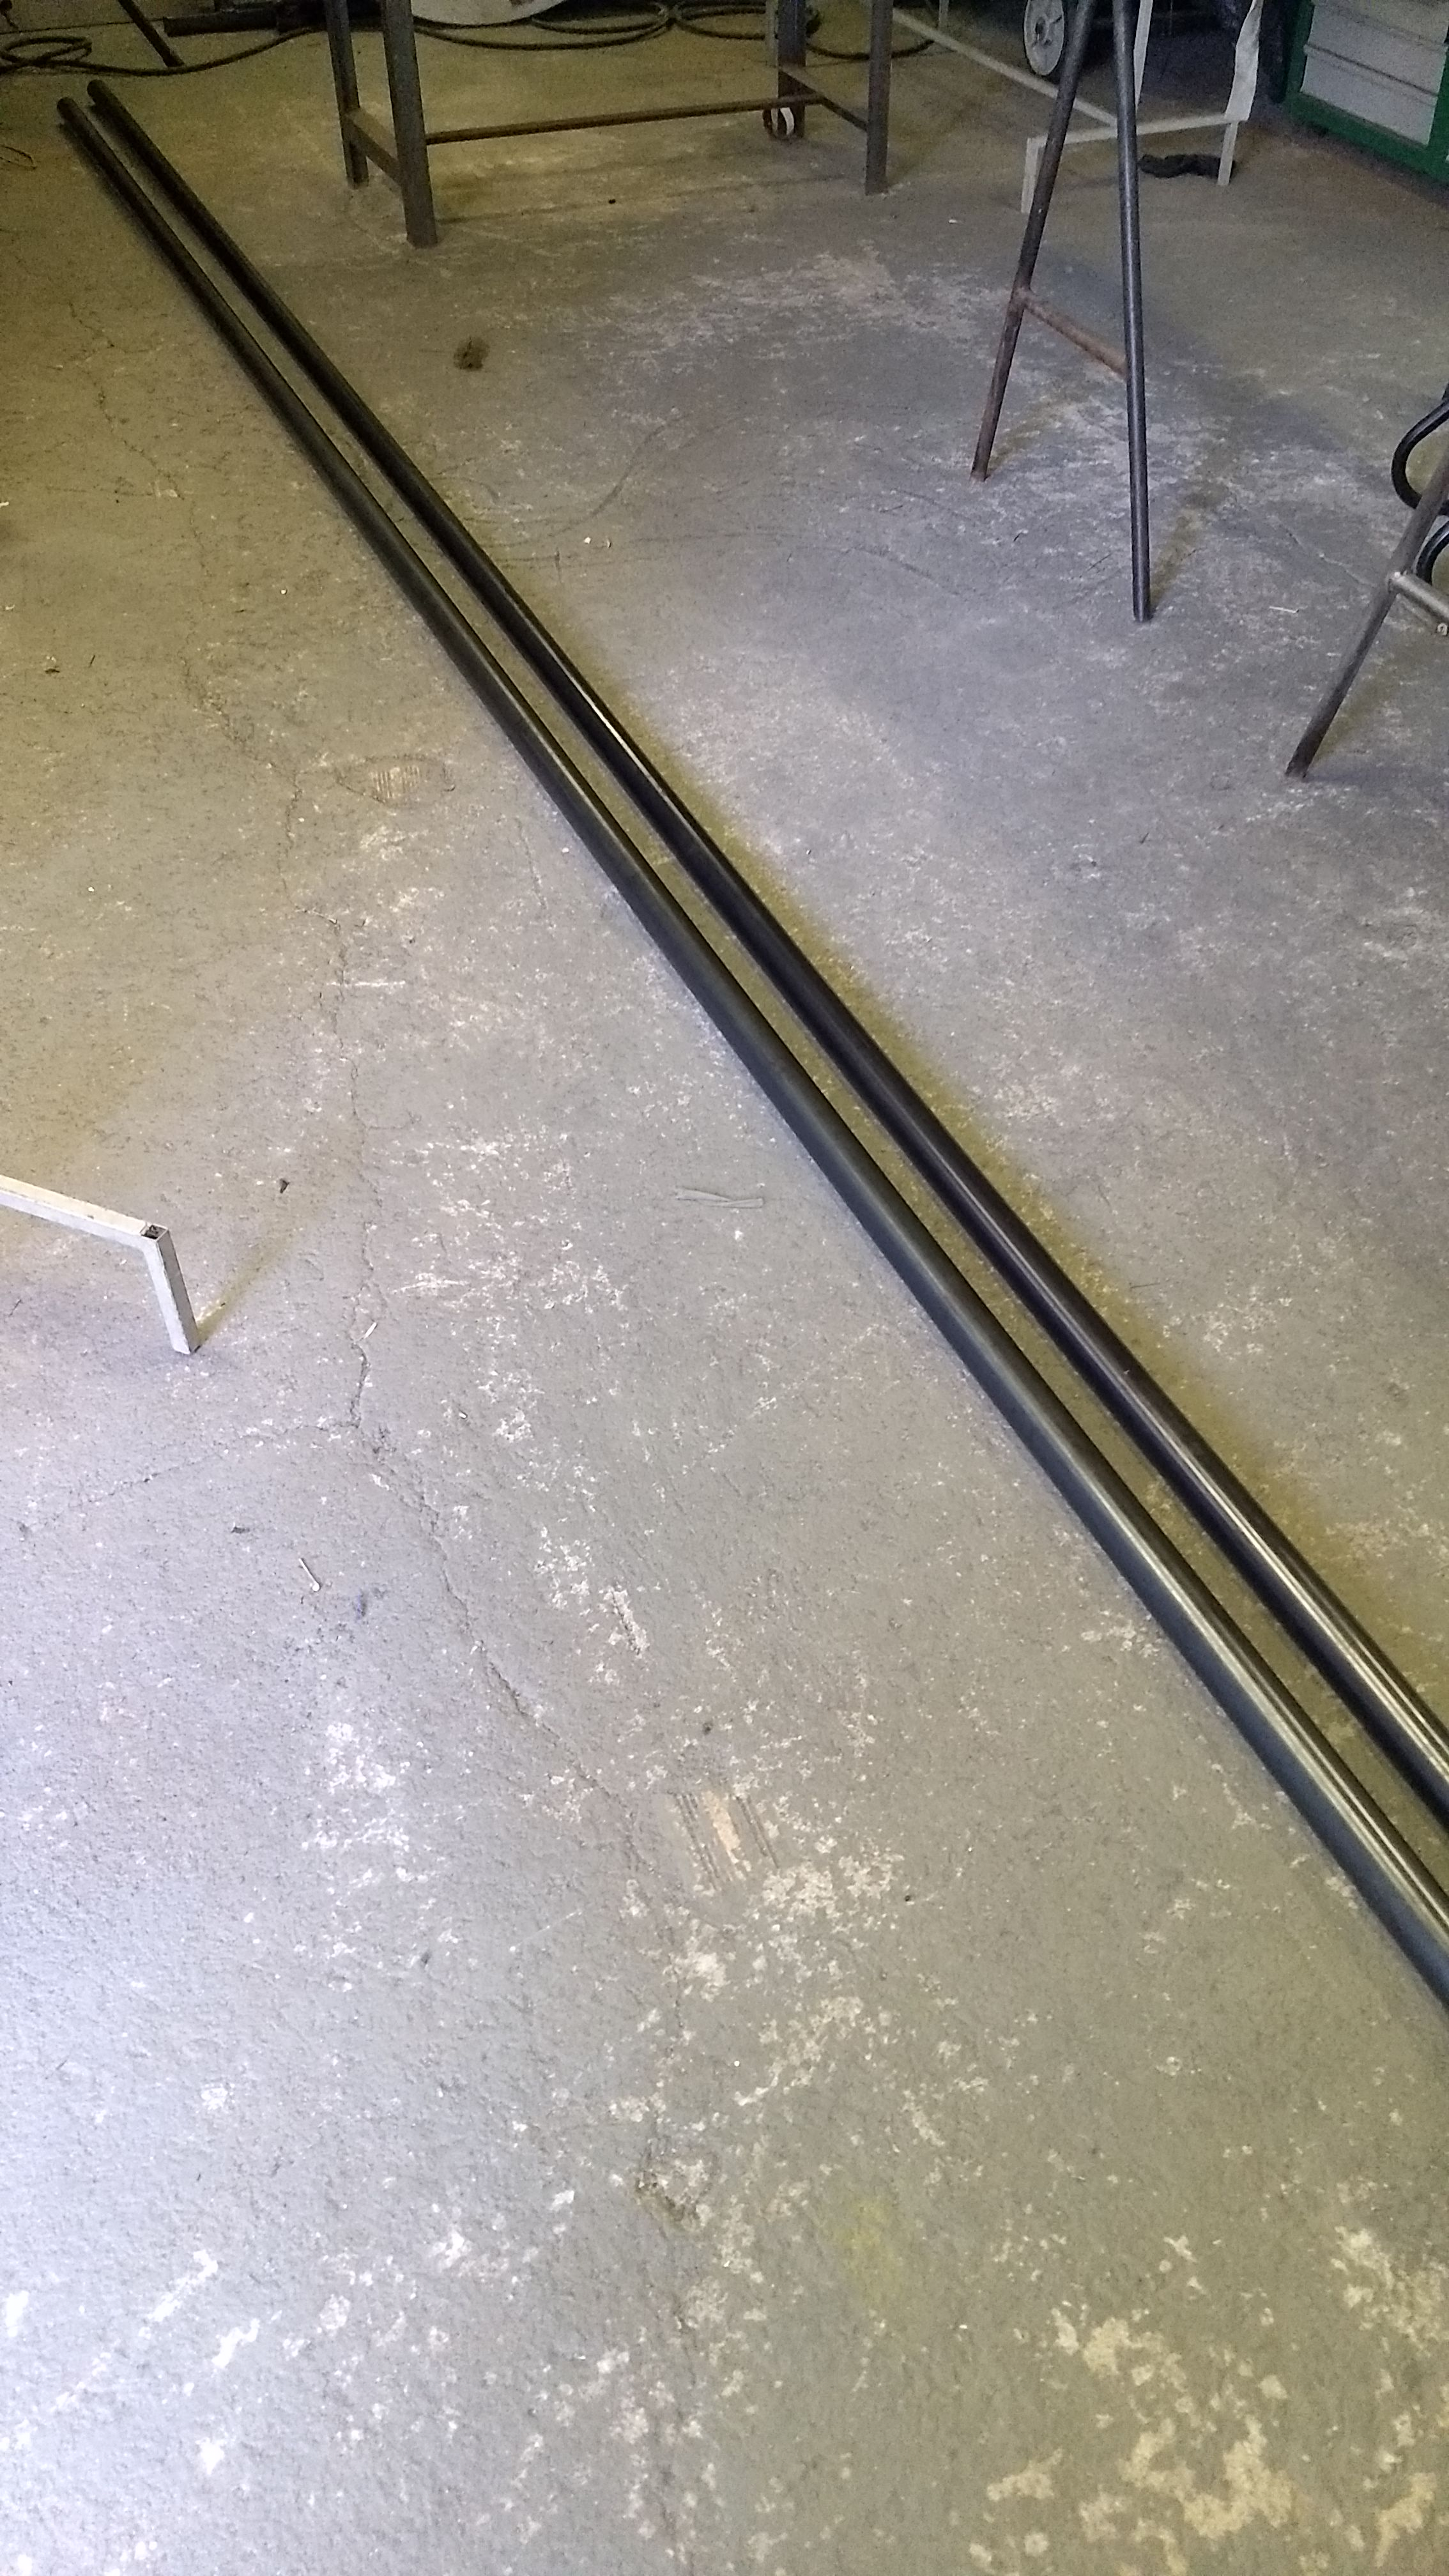
\includegraphics[keepaspectratio=true,scale=0.1,angle=90]{figuras/tubos.jpeg}
    \caption{Tubos de aço carbono chapa 13 utilizada para o projeto.}
    \label{tubos}
\end{figure}

Foram usadas 8 abraçadeiras tipo copo com 1,5 polegadas para prender as caixas nos tubos feitas de aço com 1mm de espessura, como mostra a Figura \ref{abrac}. A utilização das abraçadeiras facilita a manutenção e evita a utilização de solda para fixar as caixas.

\begin{figure}[H]
	\centering
    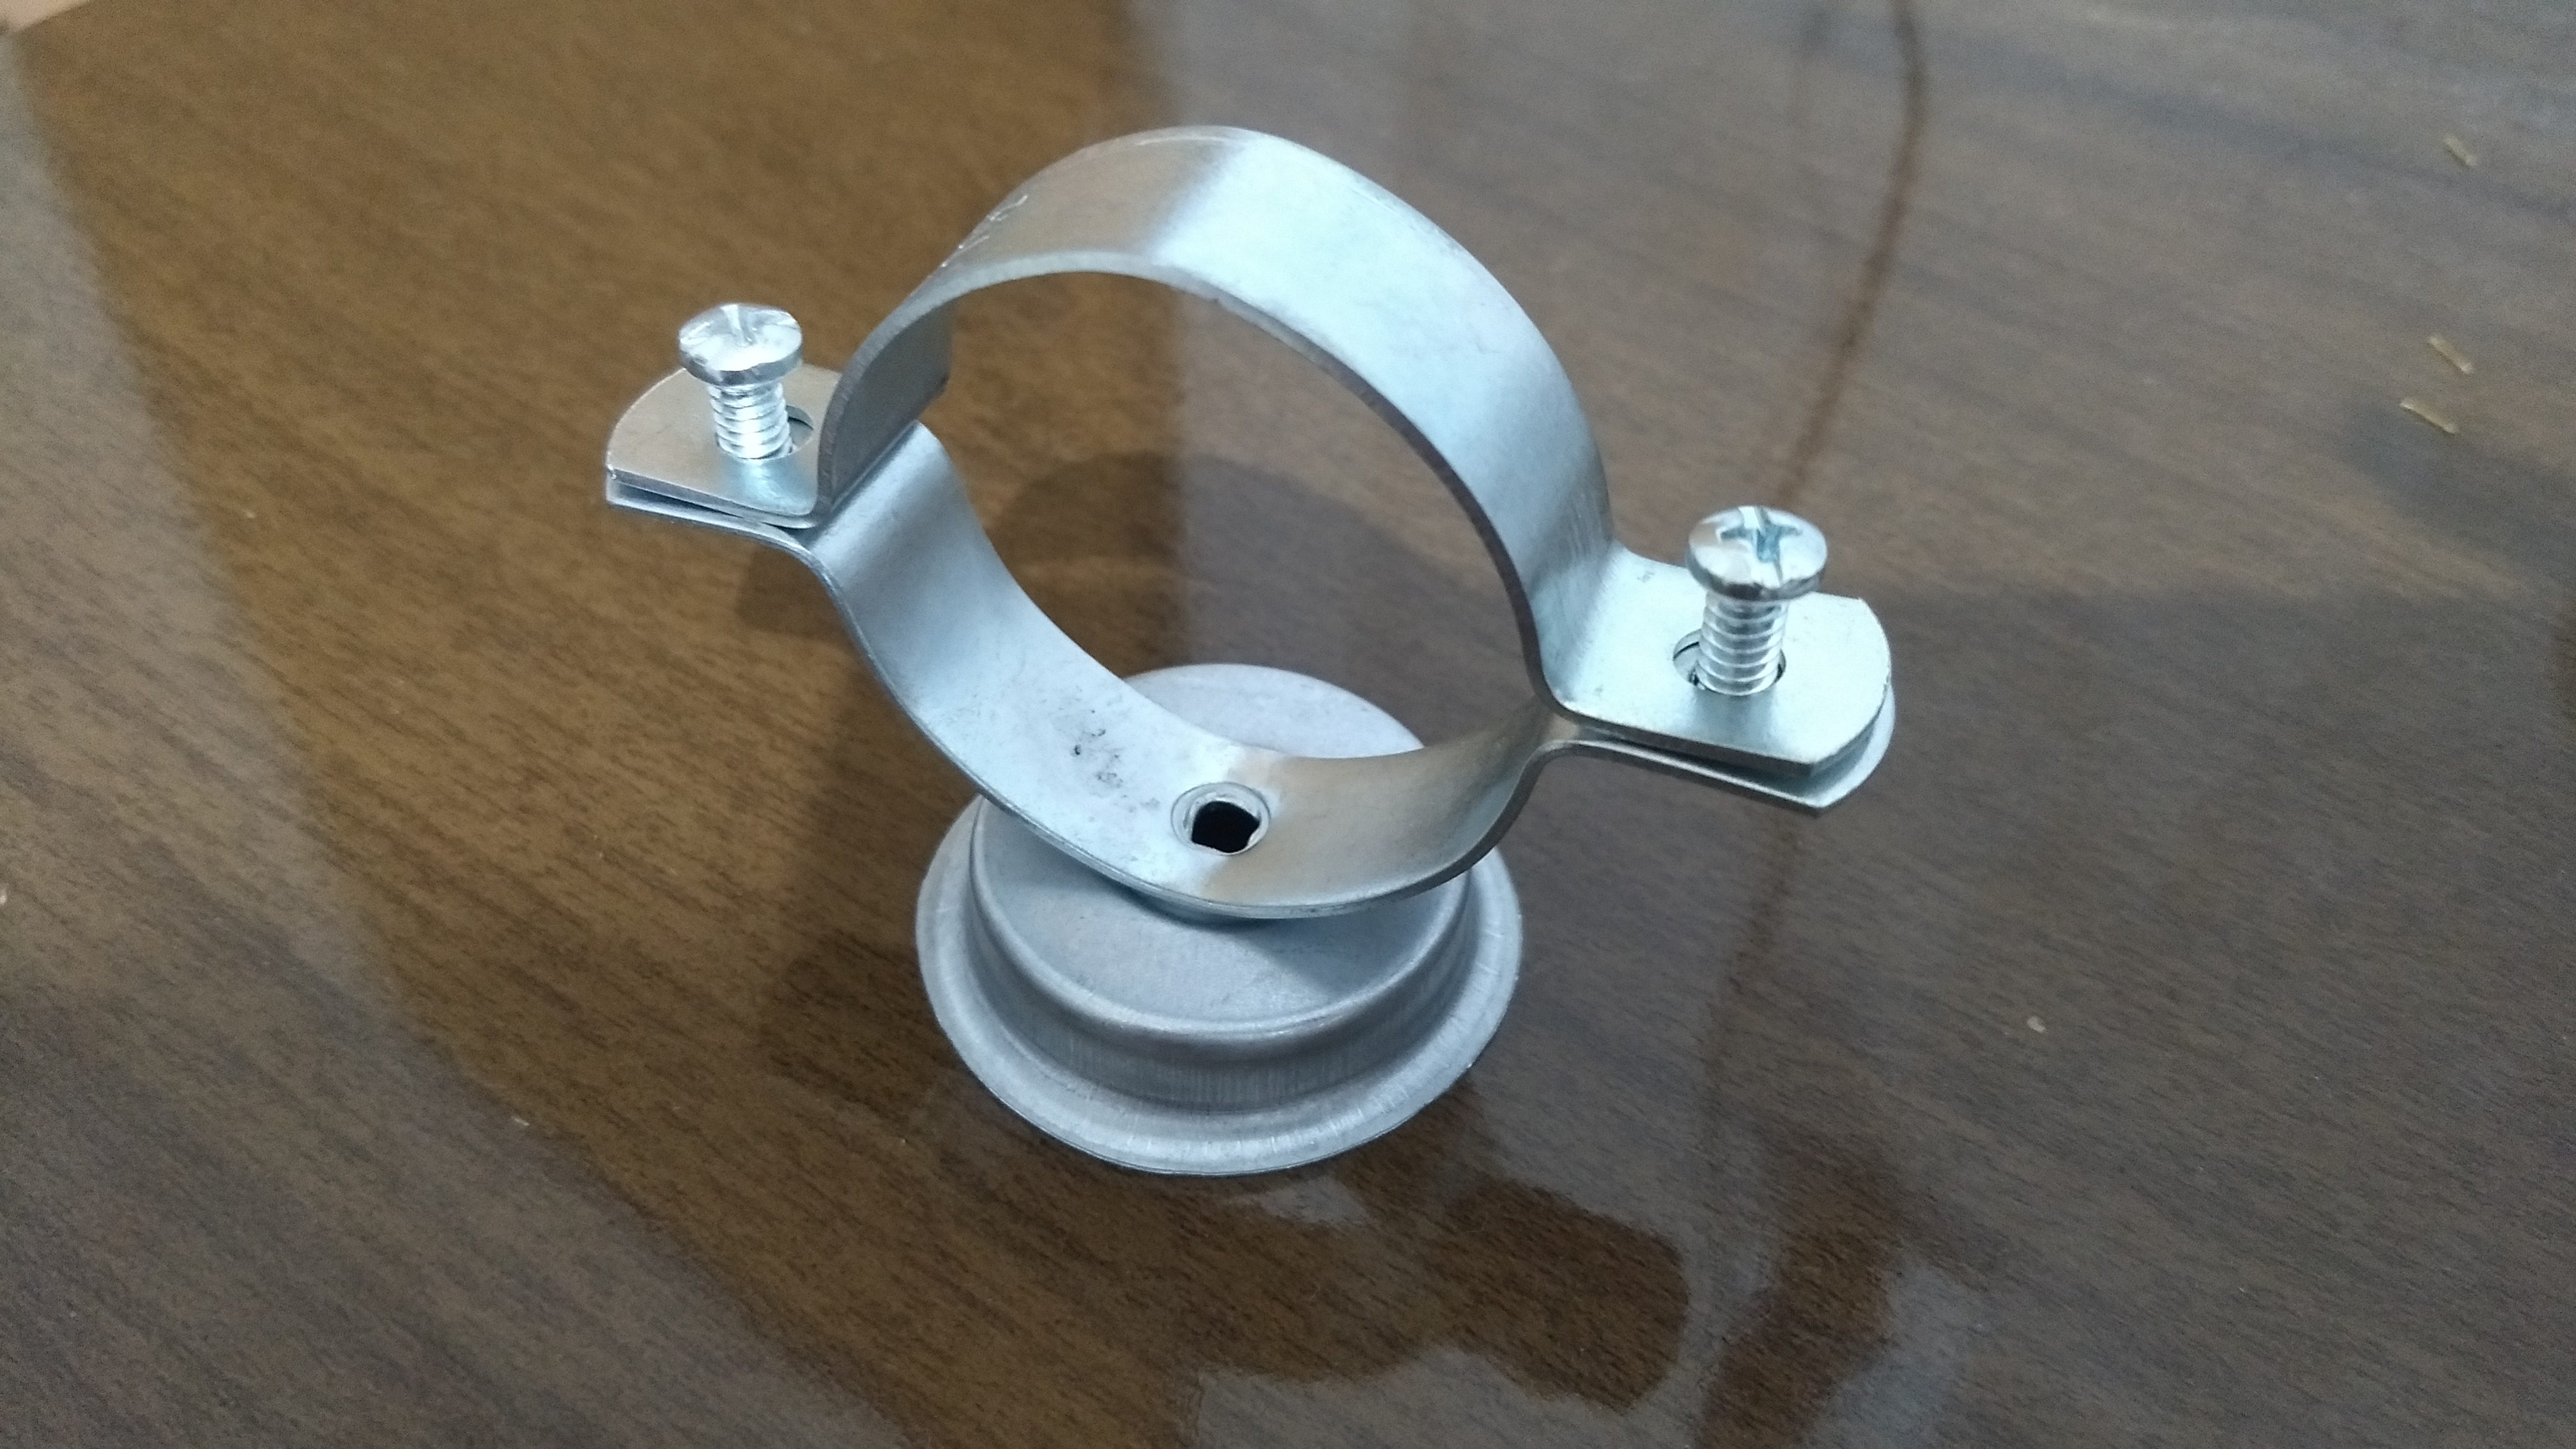
\includegraphics[keepaspectratio=true,scale=0.1]{figuras/abrac.jpg}
    \caption{Caixa de aço utilizada para o projeto.}
    \label{abrac}
\end{figure}

O suporte para o acoplamento dos painéis solares foram feitos utilizando tubos quadrados com 20mm de lado e 1,25mm de espessura de parede, como mostra a Figura \ref{tuboquad}. Foi decidido a utilização do tubo quadrado pois esse resiste melhor a flexão. Esta será feita devido o peso dos painéis solares após a instalação. Será utilizados parafusos para fixar os painéis e não permitir a queda dos mesmos. 

\begin{figure}[H]
	\centering
    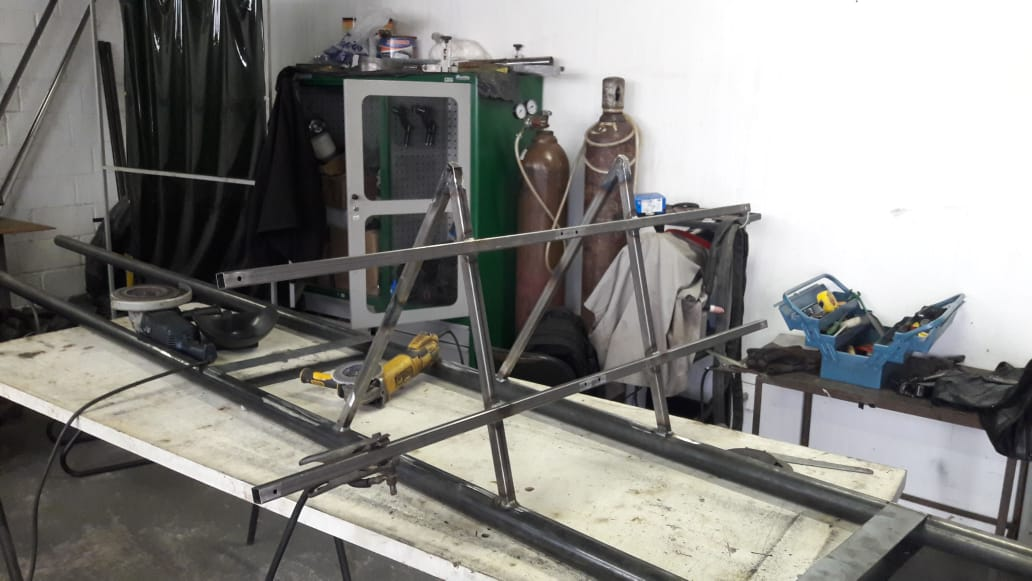
\includegraphics[keepaspectratio=true,scale=0.3]{figuras/suporte_painel_feito}
    \caption{Suporte para o acoplamento dos painéis solares feito com tubos quadrados.}
    \label{tuboquad}
\end{figure}

\subsection{Fundação}

A fundação foi pensada para proporcionar maior estabilidade para a estrutura. Ter uma fundação faz com que o protótipo esteja muito mais perto da situação do produto real. Através do aval dos responsáveis na Universidade de Brasília, será possível a construção de uma fundação de concreto no estacionamento para teste e apresentação do projeto para os professores avaliadores. 

As dimensões escolhidas para a construção da fundação são de 40x70cm na superfície e 50cm de profundidade abaixo do chão. Levando em consideração que 1 metro da estrutura (as hastes) será encaixada na fundação, 50cm será de terra e 50cm de concreto, sendo o suficiente para garantir a estabilidade necessária para a estrutura.

O local escolhido em comum acordo entres os diretores técnicos de cada subsistema proporciona um teste com melhor acurácia e mais próximo possível da realidade do problema no qual o RaDop se propõe em resolver. 

\section{Construção do Protótipo}

Inicialmente o projeto começou com a construção do suporte principal, as hastes de aço carbono. Assim foram soldados as chapas chatas entre os tubos nas dimensões corretas para criar o que será a base se sustentação de todos os demais componentes, estruturais ou não, como mostra a Figura \ref{hastescons}.

\begin{figure}[H]
	\centering
    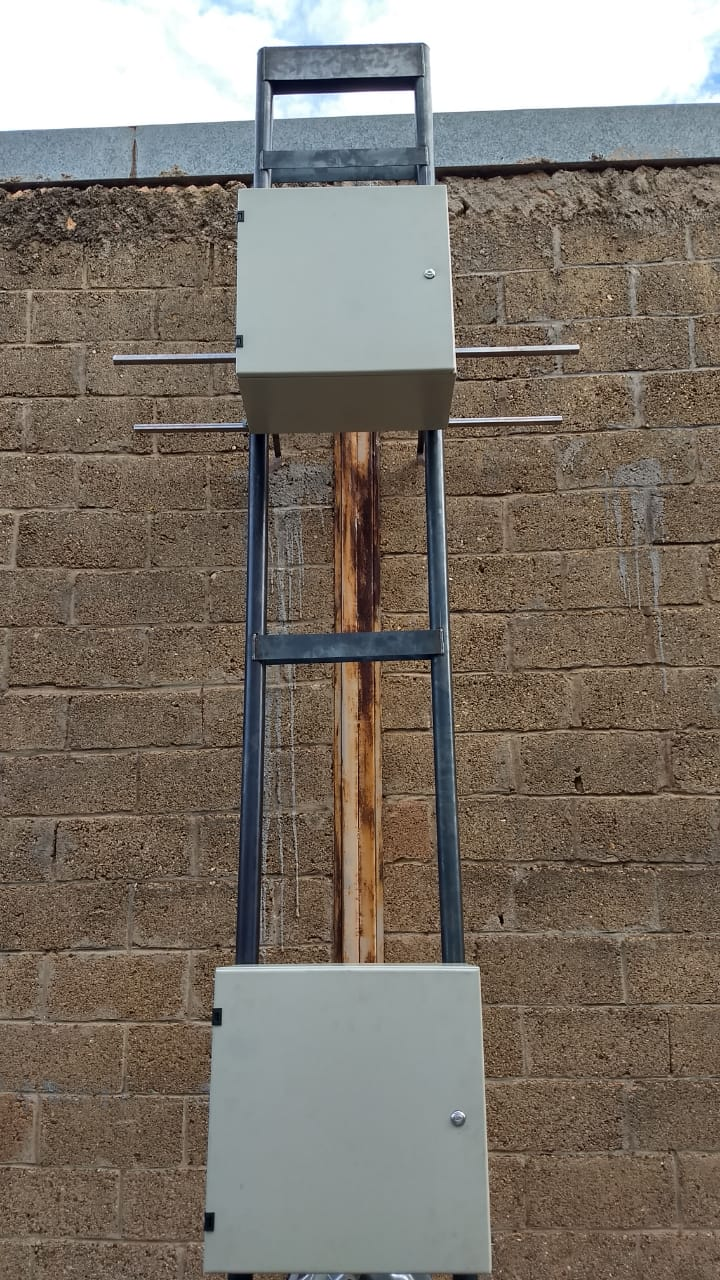
\includegraphics[keepaspectratio=true,scale=0.25]{figuras/estrutura_completa}
    \caption{Hastes construídas em aço carbono.}
    \label{hastescons}
\end{figure}

Com as hastes prontas foi então construído o último módulo que seria soldado, o suporte dos painéis solares. O corte dos tubos quadrados nas dimensões necessárias foram realizados para então soldar junto as hastes. Os furos para o encaixe dos painéis solares também foram feitos no suporte, como mostra a Figura \ref{supaisolcons}.

\begin{figure}[H]
	\centering
    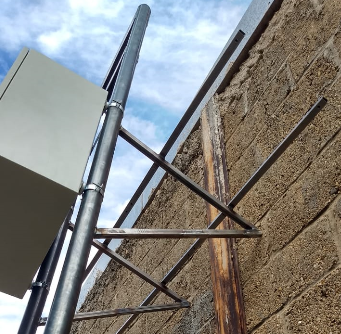
\includegraphics[keepaspectratio=true,scale=0.8]{figuras/suporte_painel2}
    \caption{Suporte dos painéis solares construídas tubos de aço carbono com 20x20mm.}
    \label{supaisolcons}
\end{figure}

Com as abraçadeiras fixadas na hastes foram feitos os furos nas placas chatas (que distribuem o peso das caixas) e nas caixas superior e inferior. Utilizando parafusos e porcas M6 foram fixadas as caixas nas alturas pré-determinadas pelos desenhos técnicos, como mostra a Figura \ref{caixaacop}.

\begin{figure}[H]
	\centering
    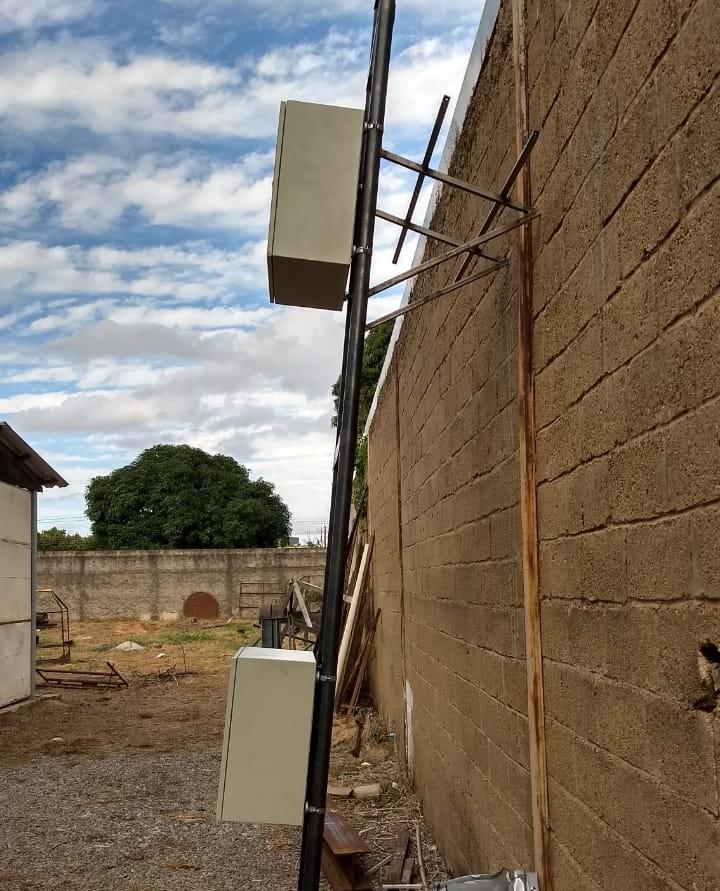
\includegraphics[keepaspectratio=true,scale=0.35]{figuras/caixa_completa_com_hastes}
    \caption{Caixa acoplada utilizando as abraçadeiras nas hastes.}
    \label{caixaacop}
\end{figure}

\section{Teste do Protótipo}

Com a estrutura pronta testes de choques mecânicos foram realizados. A estrutura foi movimentada bruscamente para ter verificar a capacidade das abraçadeiras de suportar o peso das caixas, principalmente a superior já que a inferior estará apoiada no chão (fundação) e não será solicitada em termos de esforços significativos.

As portas foram testadas para verificar se a aberturas das mesmas se davam de forma facilitada ou não. Através dos choques mecânicos realizados com a estrutura em sua posição real foram verificadas as soldas realizadas para ver se alguma ruptura havia acontecido e se o sistema poderia ser comprometido por isso.

A estrutura foi posta em inclinação para testar a possibilidade de deflexão nas hastes assim como a possibilidade de ruptura das abraçadeiras.

\section{Avaliação dos Resultados}

Através dos testes realizados a estrutura se mostrou estável. Não foi encontrado nenhuma ruptura de solda mesmo após os choques mecânicos realizados. As abraçadeiras suportaram e não mostraram nenhum sinal de mal funcionamento. As caixas se mostraram eficientes e capazes de realizar seu papel de assegurar o funcionamento dos componentes dos demais subsistemas do projeto.

Sendo assim é possível afirmar que não foi possível verificar nenhum problema que coloque a estrutura completa em risco de ruptura e mal funcionamento. Foi então confirmado experimentalmente os dados obtidos pelas simulações realizadas nas etapas anteriores do projeto.

\section{Custos}

Um levantamento orçamentário foi feito para a compra do material de construção do RaDop. Os custos aqui apresentados foram feitos através de contato com os fornecedores. 

\begin{table}[H]
\centering
\resizebox{\textwidth}{!}{%
\begin{tabular}{|c|c|c|c|c|}
\hline
\multicolumn{5}{|c|}{Estrutura} \\ \hline
Quantidade & Material & Valor Unitário & Total & Fornecedor \\ \hline
2 & Caixa Para Painel Eletrico de Aço – 500x500x250mm$^3$ & R\$ 240,00 & R\$ 480,00 & Soma \\ \hline
2 & Tubo Aço Carbono \#13 6m 2" 2,25mm & R\$ 105,24 & R\$ 210,48 & Perfibraz \\ \hline
4 & Barra Chata \#13 450x60mm$^2$ & R\$ 12,00 & R\$ 48,00 & Perfibraz \\ \hline
4 & Barra Chata \#13 486x40mm$^2$ & R\$ 12,00 & R\$ 48,00 & Perfibraz \\ \hline
2 & Barra Chata \#13 450x120mm$^2$ & R\$ 22,00 & R\$ 44,00 & Perfibraz \\ \hline
1 & Barra Chata \#13 500,8x50,8mm$^2$ & R\$ 13,30 & R\$ 13,30 & Perfibraz \\ \hline
1 & Tubo Quadrado 200x200mm$^2$ \#18 6m & R\$ 27,00 & R\$ 27,00 & Perfibraz \\ \hline
2 & Mão de Obra - Soldador & R\$ 50,00 & R\$ 100,00 & UnB \\ \hline
20 & Parafuso M6 & R\$ 1,00 & R\$ 20,00 & Líder \\ \hline
20 & Rosca M6 & R\$ 1,00 & R\$ 20,00 & Líder \\ \hline
8 & Abraçadeira Tipo Copo Horizontal 1,5" & R\$ 2,60 & R\$ 20,80 & Líder \\ \hline
1 & Cooler 120mm Led Ring Pc Gamer Fan & R\$ 58,80 & R\$ 58,80 & Mercado Livre \\ \hline
Descontos & - - & - - & R\$ 43,78 & - - \\ \hline
TOTAL & - - & - - & R\$ 1.046,60 & - - \\ \hline
\end{tabular}%
}
\caption{Custos dos materiais para a estrutura}
\label{custosestruturas}
\end{table}
